
\documentclass[border=10pt, 12pt]{standalone}
\usepackage[svgnames]{xcolor}
\usepackage{amsmath}
\usepackage{pgfplots}
\pgfplotsset{compat=newest}
\usepackage[sfdefault]{FiraSans}
\usepackage{FiraMono}
\renewcommand*\familydefault{\sfdefault}
\begin{document}
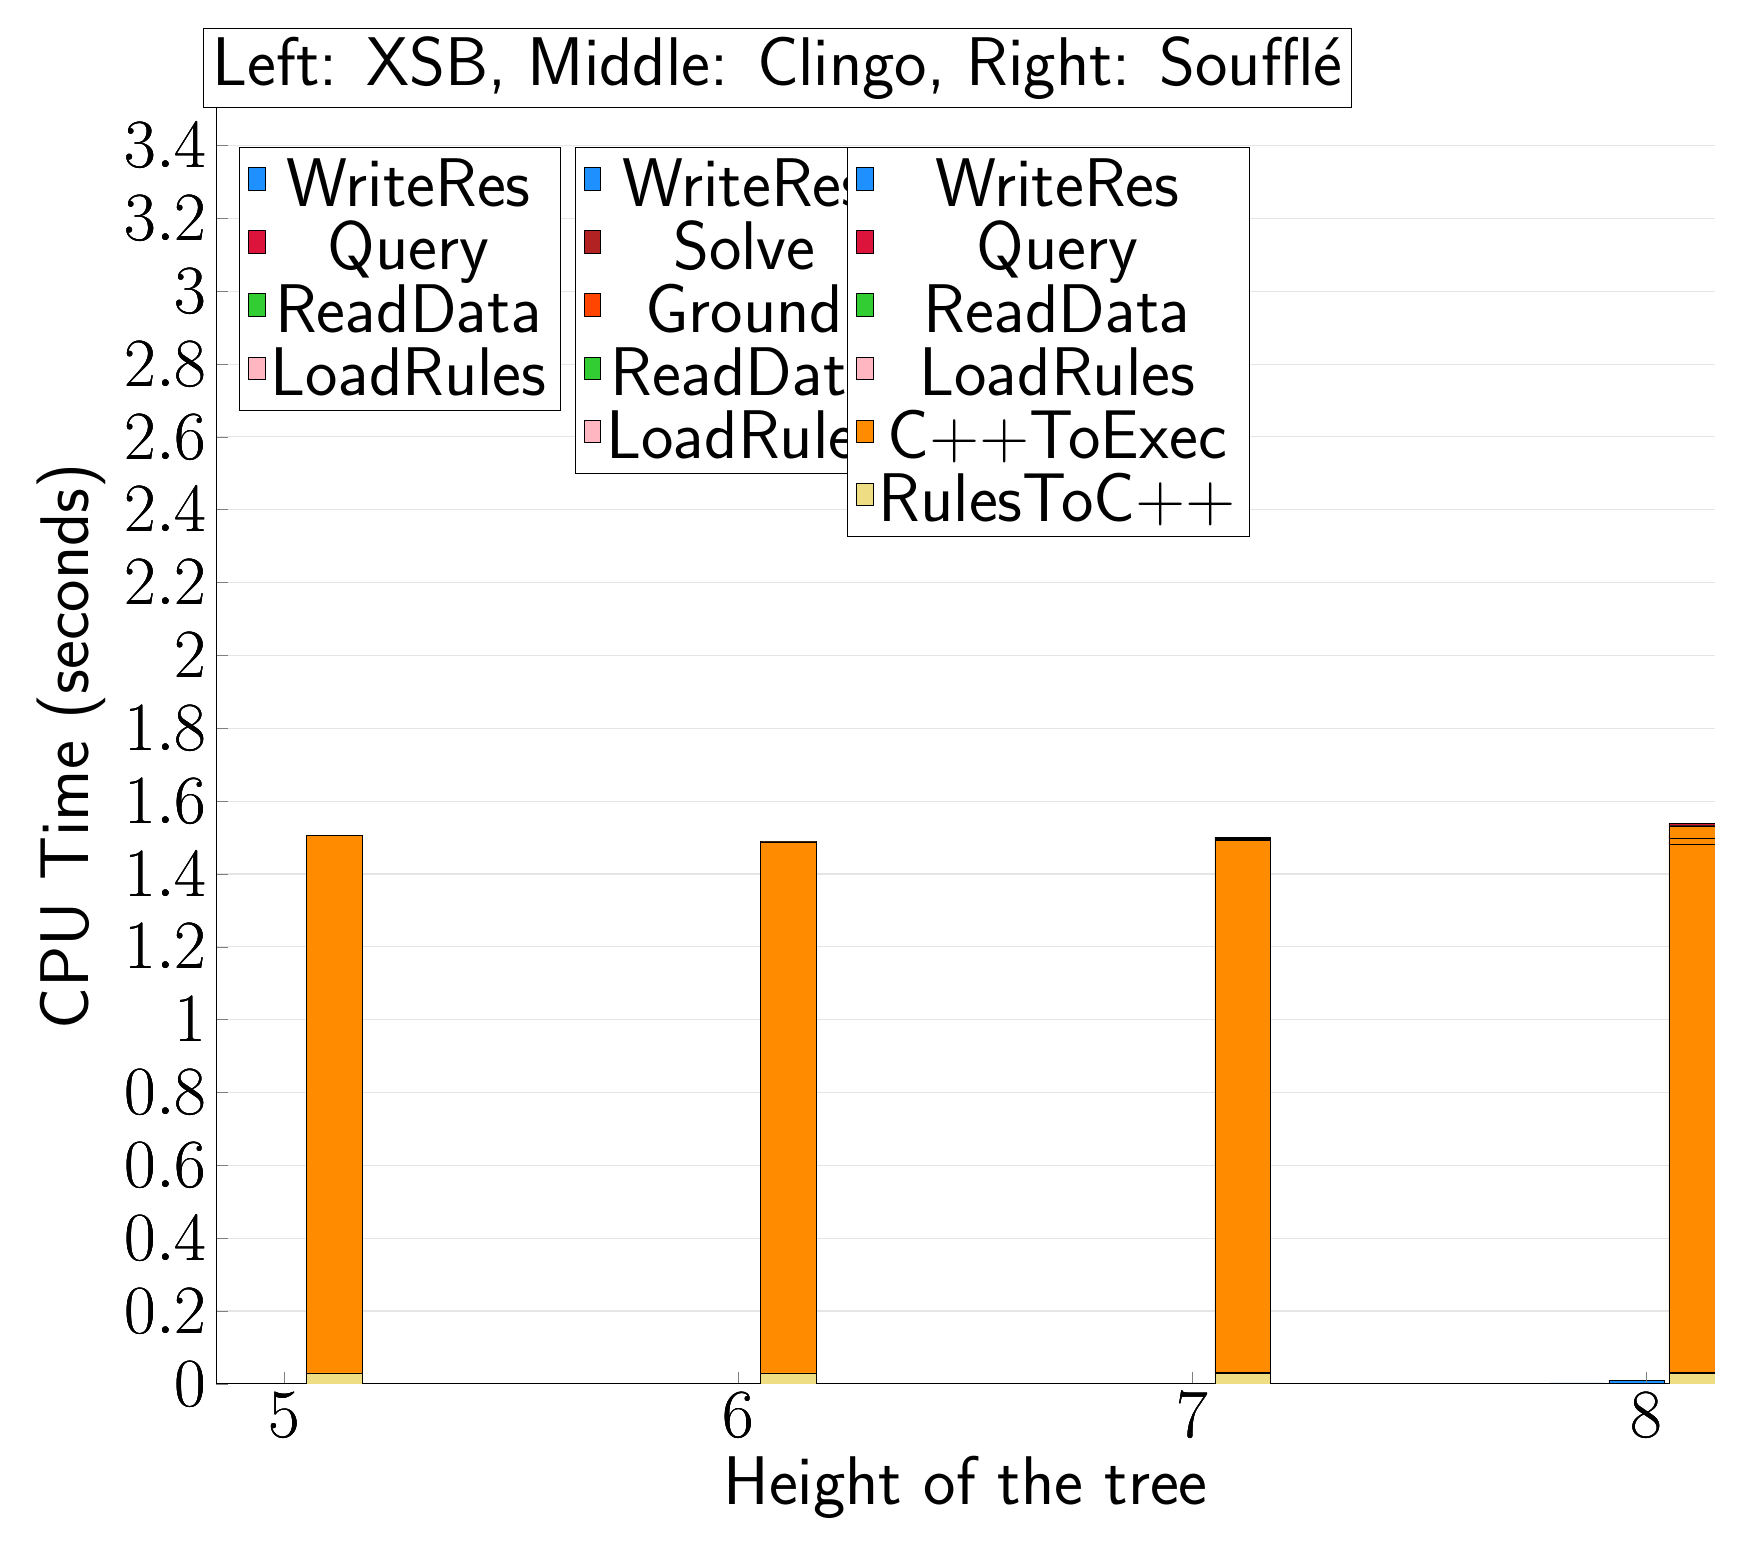
\begin{tikzpicture}
	\begin{axis}[bar shift=-25pt,
			ybar stacked,
			width=1.7\textwidth,
			bar width=0.7cm,
			ymajorgrids, tick align=inside,
			major grid style={draw=gray!20},
			xtick=data,
			ymin=0, ymax=3.5020000000000002,
			axis x line*=bottom,
			axis y line*=left,
			enlarge x limits=0.05,
			legend style={
					at={(0.23, 0.97)},
					anchor=north east,
					legend columns=1,
					font=\Huge,
				},
			ylabel={CPU Time (seconds)},
			xlabel={Height of the tree},
			label style={font=\Huge},
			tick label style={font=\Huge},
		]
		\addlegendimage{fill=DodgerBlue, draw=black, line width=0.2pt}
		\addlegendentry{WriteRes}
		\addlegendimage{fill=Crimson, draw=black, line width=0.2pt}
		\addlegendentry{Query}
		\addlegendimage{fill=LimeGreen, draw=black, line width=0.2pt}
		\addlegendentry{ReadData}
		\addlegendimage{fill=LightPink, draw=black, line width=0.2pt}
		\addlegendentry{LoadRules}
		\addplot +[fill=LightPink, draw=black, line width=0.2pt] coordinates {
				(5, 0.0006029000000000001)
				(6, 0.0006119999999999998)
				(7, 0.0006027999999999999)
				(7, 0.0006178999999999999)
				(7, 0.0006127000000000001)
				(8, 0.0006044000000000004)
				(8, 0.0006211000000000003)
				(8, 0.0006079999999999998)
			};
		\addplot +[fill=LimeGreen, draw=black, line width=0.2pt] coordinates {
				(5, 0.0001550999999999999)
				(6, 0.00018570000000000018)
				(7, 0.00024310000000000022)
				(7, 0.00024140000000000007)
				(7, 0.00024150000000000018)
				(8, 0.0003522999999999995)
				(8, 0.0003447999999999998)
				(8, 0.0003491000000000001)
			};
		\addplot +[fill=Crimson, draw=black, line width=0.2pt] coordinates {
				(5, 3.009999999999974e-05)
				(6, 6.329999999999964e-05)
				(7, 0.00015109999999999988)
				(7, 0.00014750000000000022)
				(7, 0.0001474999999999999)
				(8, 0.0003725000000000001)
				(8, 0.00036830000000000055)
				(8, 0.0003709999999999997)
			};
		\addplot +[fill=DodgerBlue, draw=black, line width=0.2pt] coordinates {
				(5, 0.00015820000000000027)
				(6, 0.00030090000000000027)
				(7, 0.0006467000000000006)
				(7, 0.0006446999999999996)
				(7, 0.0006536999999999999)
				(8, 0.0014425)
				(8, 0.0014566999999999996)
				(8, 0.0014952000000000001)
			};
	\end{axis}

	\begin{axis}[bar shift=-3.7pt,
			ybar stacked,
			width=1.7\textwidth,
			bar width=0.7cm,
			ymajorgrids, tick align=inside,
			major grid style={draw=none},
			xtick=data,
			ymin=0, ymax=3.5020000000000002,
			axis x line*=none,
			axis y line*=none,
			enlarge x limits=0.05,
			legend style={
					at={(0.454, 0.97)},
					anchor=north east,
					legend columns=1,
					font=\Huge,
				},
			label style={font=\Huge},
			tick label style={font=\Huge},
		]
		\addlegendimage{fill=DodgerBlue, draw=black, line width=0.2pt}
		\addlegendentry{WriteRes}
		\addlegendimage{fill=FireBrick, draw=black, line width=0.2pt}
		\addlegendentry{Solve}
		\addlegendimage{fill=OrangeRed, draw=black, line width=0.2pt}
		\addlegendentry{Ground}
		\addlegendimage{fill=LimeGreen, draw=black, line width=0.2pt}
		\addlegendentry{ReadData}
		\addlegendimage{fill=LightPink, draw=black, line width=0.2pt}
		\addlegendentry{LoadRules}
		\addplot +[fill=LightPink, draw=black, line width=0.2pt] coordinates {
				(5, 0.0)
				(6, 0.0)
				(7, 0.0)
				(7, 0.0)
				(7, 0.0)
				(8, 0.0)
				(8, 0.0)
				(8, 0.0)
			};
		\addplot +[fill=LimeGreen, draw=black, line width=0.2pt] coordinates {
				(5, 0.0)
				(6, 0.0)
				(7, 0.0)
				(7, 0.0)
				(7, 0.0)
				(8, 0.0)
				(8, 0.0)
				(8, 0.0)
			};
		\addplot +[fill=OrangeRed, draw=black, line width=0.2pt] coordinates {
				(5, 0.0)
				(6, 0.0)
				(7, 0.0)
				(7, 0.0)
				(7, 0.0)
				(8, 0.0)
				(8, 0.0)
				(8, 0.0)
			};
		\addplot +[fill=FireBrick, draw=black, line width=0.2pt] coordinates {
				(5, 0.0)
				(6, 0.0)
				(7, 0.0)
				(7, 0.0)
				(7, 0.0)
				(8, 0.0)
				(8, 0.0)
				(8, 0.0)
			};
		\addplot +[fill=DodgerBlue, draw=black, line width=0.2pt] coordinates {
				(5, 0.0)
				(6, 0.0)
				(7, 0.0)
				(7, 0.0)
				(7, 0.0)
				(8, 0.009999999999999997)
				(8, 0.009999999999999997)
				(8, 0.009999999999999997)
			};
	\end{axis}

	\begin{axis}[bar shift=18pt,
			ybar stacked,
			width=1.7\textwidth,
			bar width=0.7cm,
			ymajorgrids, tick align=inside,
			major grid style={draw=none},
			xtick=data,
			ymin=0, ymax=3.5020000000000002,
			axis x line*=none,
			axis y line*=none,
			enlarge x limits=0.05,
			legend style={
					at={(0.69, 0.97)},
					anchor=north east,
					legend columns=1,
					font=\Huge,
				},
			label style={font=\Huge},
			tick label style={font=\Huge},
		]
		\addlegendimage{fill=DodgerBlue, draw=black, line width=0.2pt}
		\addlegendentry{WriteRes}
		\addlegendimage{fill=Crimson, draw=black, line width=0.2pt}
		\addlegendentry{Query}
		\addlegendimage{fill=LimeGreen, draw=black, line width=0.2pt}
		\addlegendentry{ReadData}
		\addlegendimage{fill=LightPink, draw=black, line width=0.2pt}
		\addlegendentry{LoadRules}
		\addlegendimage{fill=DarkOrange, draw=black, line width=0.2pt}
		\addlegendentry{C++ToExec}
		\addlegendimage{fill=LightGoldenrod, draw=black, line width=0.2pt}
		\addlegendentry{RulesToC++}
		\addplot +[fill=LightGoldenrod, draw=black, line width=0.2pt] coordinates {
				(5, 0.030000000000000006)
				(6, 0.030000000000000006)
				(7, 0.031000000000000007)
				(7, 0.030000000000000006)
				(7, 0.030000000000000006)
				(8, 0.030000000000000006)
				(8, 0.031000000000000007)
				(8, 0.030000000000000006)
			};
		\addplot +[fill=DarkOrange, draw=black, line width=0.2pt] coordinates {
				(5, 1.4760000000000002)
				(6, 1.4579999999999997)
				(7, 1.4659999999999997)
				(7, 1.465)
				(7, 1.4620000000000002)
				(8, 1.5020000000000002)
				(8, 1.467)
				(8, 1.4509999999999996)
			};
		\addplot +[fill=LightPink, draw=black, line width=0.2pt] coordinates {
				(5, 0.00011860000000000002)
				(6, 8.8e-05)
				(7, 9.92e-05)
				(7, 9.96e-05)
				(7, 6.82e-05)
				(8, 7.439999999999999e-05)
				(8, 0.0001104)
				(8, 0.0001098)
			};
		\addplot +[fill=LimeGreen, draw=black, line width=0.2pt] coordinates {
				(5, 0.0002906)
				(6, 0.00040349999999999994)
				(7, 0.0005455)
				(7, 0.0005363)
				(7, 0.0004936)
				(8, 0.0007706000000000001)
				(8, 0.0008191)
				(8, 0.0008298000000000001)
			};
		\addplot +[fill=Crimson, draw=black, line width=0.2pt] coordinates {
				(5, 0.0002662)
				(6, 0.0008383999999999999)
				(7, 0.0022268)
				(7, 0.0022058999999999994)
				(7, 0.0019904)
				(8, 0.005409000000000001)
				(8, 0.0057082)
				(8, 0.0058922)
			};
		\addplot +[fill=DodgerBlue, draw=black, line width=0.2pt] coordinates {
				(5, 0.00026849999999999997)
				(6, 0.0003728)
				(7, 0.0005154000000000001)
				(7, 0.0005147999999999999)
				(7, 0.0004741)
				(8, 0.0008629999999999998)
				(8, 0.0009075)
				(8, 0.0009140999999999999)
			};
	\end{axis}


	\node[anchor=south, draw, fill=white] at (rel axis cs:0.42,1) {\Huge Left: XSB, Middle: Clingo, Right: Soufflé};
\end{tikzpicture}
\end{document}
